\chapter{A first approach to Hilbertian correlations}\label{parBasicHilbertianDecorrelations}%
\addcontentsline{itc}{chapter}{\protect\numberline{\thechapter}A first approach to Hilbertian correlations}

\section{Definition and first properties}\label{parDefinition}

\subsection{Equivalent definitions}

\begin{Def}\label{def4393}
Let~$(\Omega,\mcal{B},\Pr)$ be a probability space.
For~$\mcal{F}, \ab \mcal{G}$ two sub-$\sigma$-algebras of~$\mcal{B}$,
the \emph{Hilbertian correlation coefficient} (or merely ``correlation'')
between~$\mcal{F}$ and~$\mcal{G}$ is defined as
\[\label{for3441} \{\mcal{F}:\mcal{G}\}
\coloneqq \sup_{\substack{f\in\ldb(\mcal{F})\setminus\{0\}\\g\in\ldb(\mcal{G})\setminus\{0\}}}
\frac{|\EE[fg]|}{\ecty(f)\ecty(g)} .\]
If the supremum in~(\ref{for3441}) is taken over an empty set,
that is, if $\mcal{F}$ or $\mcal{G}$ is trivial,
we define this supremum to be $0$.
\end{Def}

\begin{Rmk}\label{rmk8718}
$\{\mcal{F}:\mcal{G}\}$ is often called the ``maximal correlation coefficient'' or ``$\rho$-mixing coefficient'' between~$\mcal{F}$ and~$\mcal{G}$, and denoted by~$\rho(\mcal{F},\mcal{G})$ (see~\cite{Bradley-review}).
\end{Rmk}

\begin{Rmk}
In other words, $\{\mcal{F}:\mcal{G}\}$ is the best $k\in\RR_+$ such that the following refined
Cauchy--Schwarz inequality holds in the Hilbert space $\ldb(\mcal{B})$:
\[ \forall f \in \ldb(\mcal{F}) \enskip\forall g \in \ldb(\mcal{G})
\qquad |\langle f,g \rangle| \leq k \|f\| \|g\| .\]

Yet another formulation is that $\{\mcal{F}:\mcal{G}\}$ is the cosine of the angle
between~$\ldb(\mcal{F})$ and~$\ldb(\mcal{G})$, seen as subspaces of~$\ldb(\mcal{B})$
—this angle being defined as the infimum angle
between any two non-zero vectors of these respective subspaces.

If we speak in terms of~$L^2$ spaces rather than $\ldb$ spaces,
$\{\mcal{F}:\mcal{G}\}$ is the best $k\in\RR_+$ such that
for all non-constant square-integrable~$f,g$ resp.\ $\mcal{F}$ and $\mcal{G}$-measurable,
\[\label{for0263} |\Corr(f,g)| \leq k ,\]
where $\Corr(f,g) \coloneqq \Cov(f,g) \div \ecty(f)\ecty(g)$ is the Pearson correlation coefficient between~$f$ and~$g$.
\end{Rmk}

\begin{Def}
We say that $\mcal{F}$ and~$\mcal{G}$ are \emph{$\epsilon$-decorrelated},
resp.\ \emph{$\epsilon$-correlated}, if $\{\mcal{F}:\mcal{G}\}\leq\epsilon$,
resp.\ $\{\mcal{F}:\mcal{G}\} \geq \epsilon$.
\end{Def}

\begin{Def}\label{def3792}
For~$X$ and~$Y$ random variables (with arbitrary ranges), we will denote~${\{X:Y\}}$
for~${\{\sigma(X):\sigma(Y)\}}$.
\end{Def}

\begin{Rmk}
One can rewrite Definition~\ref{def3792} as
\[\label{for3878}
\{ X:Y \} = \sup_{f,g} \frac{\Cov\big( f(X), g(Y) \big)}{\ecty\big(f(X)\big)\ecty\big(g(Y)\big)} ,\]
where it is implied that $f$ and~$g$ have to be measurable, real,
and such that $0 < \ecty(f(X)), \ab \ecty(g(Y)) \ab {< \infty}$.
\end{Rmk}

\begin{NOTA}
More generally, all the questions relative to Hilbertian correlations
may be handled either in terms of $\sigma$-algebras or in terms of random variables.
In the sequel, we will frequently switch implicitly between these two paradigms.
\end{NOTA}

It is natural to enquire what happens if one deals with \emph{complex} $\ldb$ spaces.
In fact it does not change anything:
\begin{Pro}[{\cite[Theorem~1.1]{Withers}}]
Let~$\mcal{F}$ and~$\mcal{G}$ be two $\sigma$-algebras
and let~$f,g$ be two complex centered $L^2$ variables,
measurable w.r.t.\ resp.~$\mcal{F}$ and~$\mcal{G}$.
Then, with~$\ecty(f)$ meaning $\sqrt{\EE[|f-\EE[f]|^2]}$, one has:
\[ |\EE[fg]| \leq \{\mcal{F}:\mcal{G}\} \ecty(f) \ecty(g) .\]
\end{Pro}
%
\begin{proof}
I recall the proof for the sake of completeness.
Up to multiplying $g$ by a well-chosen unit complex number,
we can assume that $\EE[fg] \ab {\in \RR_+}$.
Then we can apply Definition~\ref{def4393} to the \emph{real} $\ldb$ variables%
~$\Re f$ and~$\Re g$, resp.~$\Im f$ and~$\Im g$, getting:
\begin{multline}
|\EE[fg]| = \Re \EE[fg] = \EE[\Re f \Re g] - \EE[\Im f \Im g] \\
\leq \{\mcal{F}:\mcal{G}\} \big( \ecty(\Re f) \ecty(\Re g) + \ecty(\Im f) \ecty(\Im g) \big) \\
\footrel{\text{CS}}{\leq} \{\mcal{F}:\mcal{G}\} \sqrt{\Var(\Re f)+\Var(\Im f)} \sqrt{\Var(\Re g)+\Var(\Im g)} \\
= \{\mcal{F}:\mcal{G}\} \ecty(f) \ecty(g).
\end{multline}
\end{proof}

Now we turn to a different way of seeing correlation levels.

\begin{Def}
For~$\mcal{F}, \mcal{G}$ two $\sigma$-algebras, we denote by~$\pi_{\mcal{G}\mcal{F}}$
the `projection' operator
\[\label{for0595} \begin{array}{rrcl} \pi_{\mcal{G}\mcal{F}} \colon & \ldb(\mcal{F}) & \to & \ldb(\mcal{G}) \\ & f & \mapsto & f^{\mcal{G}}. \end{array} \]

For~$\mcal{F}, \ldots, \mcal{Z}$ $\sigma$-algebras,
we denote $\pi_{\mcal{Z}\mcal{Y}\mcal{X}\ldots\mcal{G}\mcal{F}} \coloneqq
\pi_{\mcal{Z}\mcal{Y}} \circ \ab \pi_{\mcal{Y}\mcal{X}} \circ \ab \cdots \circ \pi_{\mcal{G}\mcal{F}}$.
\end{Def}

With this vocabulary at hand,
\begin{Pro}\label{pro7764}
For~$\mcal{F}, \mcal{G}$ two $\sigma$-algebras, $\{\mcal{F}:\mcal{G}\} = \VERT \pi_{\mcal{G}\mcal{F}} \VERT$.
\end{Pro}

\begin{proof}
$\pi_{\mcal{G}\mcal{F}}$ is the orthogonal projection from $\ldb(\mcal{F})$
to~$\ldb(\mcal{G})$ in the Hilbert space $\ldb(\mcal{B})$,
so its norm is the cosine of the angle between~$\ldb(\mcal{F})$ and~$\ldb(\mcal{G})$,
i.e.\ ${\{\mcal{F}:\mcal{G}\}}$.
\end{proof}

\begin{Rmk}\label{rmk1265}
One has $\pi_{\mcal{F}\mcal{G}} = \pi_{\mcal{G}\mcal{F}}^*$,
since $\langle \pi_{\mcal{G}\mcal{F}}f , g \rangle = \EE[fg] = \langle f , \pi_{\mcal{F}\mcal{G}}g \rangle$.
Therefore the expression $\VERT \pi_{\mcal{G}\mcal{F}} \VERT$ in Proposition~\ref{pro7764}
can be rewritten into $\sqrt{\VERT \pi_{\mcal{F}\mcal{G}\mcal{F}} \VERT}$,
which is also $\rho(\pi_{\mcal{F}\mcal{G}\mcal{F}})$
since $\pi_{\mcal{F}\mcal{G}\mcal{F}}$ is self-adjoint.
\end{Rmk}



\subsection{Immediate properties}

Having defined Hilbertian correlations, it is now time to study their behaviour.

The following properties are immediate from Definition~\ref{def4393}:
%
\begin{Pro}
For all $\sigma$-algebras $\mcal{F}$, $\mcal{G}$ and~$\mcal{G}'$,
\begin{ienumerate}
\item $\{\mcal{G}:\mcal{F}\} = \{\mcal{F}:\mcal{G}\}$;
\item $\mcal{G}\subset\mcal{G}' \ \Rightarrow\ \{\mcal{F}:\mcal{G}\} \leq \{\mcal{F}:\mcal{G}'\}$;
\item $\{\mcal{F}:\mcal{G}\} \in [0,1]$;
\item $\{\mcal{F}:\mcal{G}\} = 0$ if and only if $\mcal{F}$ and~$\mcal{G}$ are independent;
\item If $\mcal{F}$ is not trivial, then $\{\mcal{F}:\mcal{F}\} = 1$.
\end{ienumerate}
\end{Pro}

When one is concerned by correlation between variables,
it often occurs that some of these variables are vector-valued.
The following proposition means
that it suffices to know the behaviour of finite-length vectors
to understand the behaviour of all vectors:
%
\begin{Pro}\label{pro6559}
Let~$I, J$ be possibly infinite sets
and let~$\vec{X}_I, \vec{Y}_J$ be vector-valued variables. Then,
denoting ``$I'\Subset I$'' to mean that $I'$ is a finite subset of~$I$,
\[ \big\{ \vec{X}_I : \vec{Y}_J \big\} =
\sup_{I'\Subset I,J'\Subset J}
\big\{ \vec{X}_{I'} : \vec{Y}_{J'} \big\} .\]
\end{Pro}

\begin{proof}
This is because $\bigcup_{I'\Subset I} \ldb(\vec{X}_{I'})$,
resp.~$\bigcup_{J'\Subset J} \ldb(\vec{X}_{J'})$,
is a dense subset of~$\ldb(\vec{X}_I)$, resp.\ $\ldb(\vec{Y}_J)$.
That property follows by classical approximation arguments
like in the proof of~\cite[Theorem~3.14]{Rudin}.
See~\cite[Theorem~3.16(II-3)]{Bradley-book} for a more detailed proof.
\end{proof}



\subsection{Operator interpretation}\label{parOperatorInterpretation}

\begin{Pro}\label{cor0706}
If $X \to Y \to Z$ is a Markov chain, then $\{X:Z\} \leq {\{X:Y\}} \* {\{Y:Z\}}$.
\end{Pro}

\begin{proof}
The Markov chain property is equivalent to meaning that $\pi_{ZX} = \pi_{ZYX}$,
so the result is a consequence of the submultiplicativity of operator norms.
See also~\cite[\S~VII-4]{Rosenblatt}.
\end{proof}

There is a refined version of Proposition~\ref{cor0706} which is particularly interesting
for reversible chains:
%
\begin{Pro}\label{pro0281}
If $X \to Y \to Z$ is a Markov chain, then $\{X:Z\} = \sqrt{\rho(\pi_{YZY}\circ\pi_{YXY})}$.
\end{Pro}

\begin{proof}
Because of the Markov chain property, $\pi_{XZ} = \pi_{XY}\circ\pi_{YZ}$
and $\pi_{ZX} = \pi_{ZY}\circ\pi_{YX}$.
Using that for any pair of operators~$\pi \colon H_1 \to H_2$ and~$\tau \colon H_2 \to H_1$
one has $\rho(\pi\circ\tau) = \rho(\tau\circ\pi)$,
we get that $\{X:Z\}^2 = \rho(\pi_{XY}) = \rho(\pi_{XYZYX}) = \rho(\pi_{XY}\circ\pi_{YZYX})
= \rho(\pi_{YZYX}\circ\pi_{XY}) = \rho(\pi_{YZY}\circ\pi_{YXY})$.\linebreak[1]\strut
\end{proof}

\begin{Cor}\label{cor5902}
If $\cdots \to X_{-1} \to X_{0} \to X_{1} \to \cdots$ is a stationary Markov chain
so that $\pi_{X_1X_0}$ and~$\pi_{X_0X_1}$ commute%
\footnote{Reversible chains always satisfy this condition
since then $\pi_{X_1X_0} = \pi_{X_0X_1}$.},
then for all~$k\in\ZZ\setminus\{0\}$, $\{X_0:X_k\} = \{X_0:X_1\}^{|k|}$.
\end{Cor}

\begin{proof}
Since the chain is stationary, all the~$X_n$ have the same law
and thus all the~$\ldb(X_n)$ can be identified;
then the stationarity property is equivalent to saying that
$\pi_{X_{n+1}X_n} = \pi_{X_1X_0}$ for all~$n\in\ZZ$.
Thanks to the commutation hypothesis, one can write for~$k>0$:
\[ \{X_0:X_k\} = \sqrt{\rho(\pi_{X_0X_kX_0})}
= \sqrt{\rho(\pi_{X_0X_1}^k\circ\pi_{X_1X_0}^k)} \\
= \sqrt{\rho(\pi_{X_0X_1X_0}^k)}
= \sqrt{\rho(\pi_{X_0X_1X_0})^k} = \{X_0:X_1\}^k . \]
For the case $k<0$, we use that $\{X_0:X_k\} = \{X_{-k}:X_0\}$.
\end{proof}



\subsection{First criteria for decorrelation}\label{parCriteriaForDecorrelation}


\paragraph{Density sufficient condition}

\begin{Pro}\label{pro0651}
Let~$X$ and~$Y$ be two random variables valued resp.\ in~$E$ and~$F$.
Suppose that $\Law(X,Y)$ has a density $h$ w.r.t.\ the product probability $\Law(X)\otimes\Law(Y)$.
Then:
\[\label{for0255} \{X:Y\} \leq \Big( \int_{E\times F} (h-1)^2 \,\dx{Law_X}\,\dx{Law_Y} \Big)^{1/2} .\]
\end{Pro}

\begin{Rmk}\label{rmk5108}
The integral expression in~(\ref{for0255})
is nothing but $2$ times the bilinearized version of the mutual information
\[\label{eq9402} I(X;Y) \coloneqq \int_{E\times F} h \ln h \,\dx{Law_X}\,\dx{Law_Y} .\]
Yet Example~\ref{x3993} will show that one does not have
${\{X:Y\}} \leq \sqrt{2} \* (X;Y)^{1/2}$ in general.
\end{Rmk}

\begin{proof}
To alleviate notation, denote resp.~$\Pr_X,\ab \Pr_Y,\ab \Pr_{(X,Y)}$ for~$\Law(X),\ab \Law(Y),\ab \Law(X,Y)$.
Let~$f$ and~$g$ be centered $L^2$~functions being resp.\ $X$- and $Y$-measurable.
Observe first that
\[ \int_{E\times F}f(x)g(y) \,\dx{\Pr_X}[x]\dx{\Pr_Y}[y] =
\Big(\int_E f \,\dx{\Pr_X}\Big) \Big(\int_F g \,\dx{\Pr_Y} \Big) = 0 \times 0 = 0 ,\]
so that
\[ \EE[fg] = \int fg \,\dx{\Pr_{(X,Y)}}
= \int hfg \,\dx{\Pr_X}\dx{\Pr_Y} = \int (h-1)fg \,\dx{\Pr_X}\dx{\Pr_Y} \]
and thus
\[\label{cal1083}
|\EE[fg]| \leq \Big( \int (h-1)^2 \,\dx{\Pr_X}\dx{\Pr_Y} \Big)^{1/2}
\Big( \int f^2 g^2 \,\dx{\Pr_X} \dx{\Pr_Y} \Big)^{1/2} \]
by the Cauchy--Schwarz inequality.
%
But the last factor in the right-hand side of~(\ref{cal1083}) is
\[ \Big( \int f^2(x) g^2(y) \,\dx{\Pr_X}[x] \dx{\Pr_Y}[y] \Big)^{1/2}
= \Big( \int f^2 \dx{\Pr_X} \Big)^{1/2}
\Big( \int g^2 \dx{\Pr_Y} \Big)^{1/2}
= \ecty(f) \ecty(g) ,\]
so that (\ref{for0255}) is proved.

You may also see \cite[Theorem~2.5]{Bryc} for an analogous result.
\end{proof}


\paragraph{Event necessary condition}

\label{parpro0699}\begin{Pro}[event necessary condition]\label{pro0699}
Let~$\mcal{F}$ and~$\mcal{G}$ be two $\sigma$-algebras.
If $\{ \mcal{F} : \mcal{G} \} \leq \epsilon$,
then for all events~$A\in\mcal{F}$ and~$B\in\mcal{G}$
with respective probabilities~$p$ and~$q$,
\[\label{for3346} \big| \Pr[A\cap B] - pq \big| \leq \epsilon \sqrt{p(1-p)q(1-q)} .\]

In particular, if there exists two non-trivial events $A\in\mcal{F}, B\in\mcal{G}$
which are equivalent (in the sense that $\Pr[A\bigtriangleup B] = 0$),
then $\{\mcal{F}:\mcal{G}\} = 1$.\footnote{%
The converse is not true: it can occur that $\{\mcal{F}:\mcal{G}\}=1$
but that no non-trivial events of~$\mcal{F}$ and~$\mcal{G}$ are equivalent.
A counterexample is the following: let~$(X_n)_{n\in\NN}$
be independent $\mathit{Bernoulli}(1/2)$ variables, and define independently
$Y_n = 1-X_n$ with probability~$\epsilon_n$ and $Y_n = X_n$ otherwise,
where $(\epsilon_n)_{n\in\NN}$ is a sequence of numbers such that
$0 < \epsilon_n \leq 1/2$ for all~$n$
and $\epsilon_n\stackrel{n\longto\infty}{\longto}0$.
Then the vectorial variables~$\vec{X}$ and~$\vec{Y}$ obviously satisfy $\{\vec{X}:\vec{Y}\} = 1$,
yet it is not hard to prove that no $\vec{X}$-measurable non-trivial event
is equivalent to a $\vec{Y}$-measurable one.}
\end{Pro}

\begin{proof}
It follows from~(\ref{for0263}) applied to~$\1{A}$ and~$\1{B}$.
\end{proof}


\subsection{Independent tensorization}\label{parIndependentTensorization}

Now we are turning to the basic tensorization theorem,
which will motivate~\S~\ref{parTensorization}:
%
\begin{Thm}[{\cite[Theorem~6.2]{CsakiFischer}}]\label{pro1252}
Let~$I$ be a set and let~$\vec{X}_I,\vec{Y_I}$ be vectorial variables.
Suppose all the pairs $(X_i,Y_i)$, $i\in I$, are independent, then
\[\label{for6560} \big\{ \vec{X} : \vec{Y} \big\} = \sup_{i\in I} \{ X_i : Y_i \} .\]
\end{Thm}

\begin{proof}
The simplest proof of Theorem~\ref{pro1252}
relies on the operator interpretation of correlations,
see e.g.\ the proof of~\cite[Theorem~1]{Witsenhausen}.
Here however I shall give a proof
based on decomposing functions of several variables into telescopic sums,
for this kind of arguments will be used again
in the proofs of the more general tensorization theorems of~\S~\ref{parTensorization}.

First, observe that the ``$\geq$'' inequality of~(\ref{for6560}) is trivial,
so we only have to prove the ``$\leq$'' inequality.
We denote $\epsilon_i \coloneqq {\{X_i:Y_i\}}$,
and to alleviate notation, $x_i$ will implicitly stand for an element in the range of~$X_i$,
resp.~$y_i$ for an element in the range of~$Y_i$.

By Proposition~\ref{pro6559}, we may assume that $I$ is finite,
say $I = \{1,\ldots,N\}$ for some $N\in\NN$.
Let~$f$ and~$g$ be resp.\ $\vec{X}_I$-measurable and $\vec{Y}_I$-measurable
centered $L^2$ real functions; our goal is to bound above $|\EE[fg]|$.

For~$i\in\{0,\ldots,N\}$, define $\mcal{F}_i \coloneqq \bigvee_{j\leq i} \sigma(X_j,Y_j)$.
I claim that, because of the independence hypothesis,
$f^{\mcal{F}_i}$ only depends on the values of~$X_1,\ldots,X_i$
and not on~$Y_1,\ldots,Y_i$, and similarly
that $g^{\mcal{F}_i}$ only depends on the values of~$Y_1,\ldots,Y_i$:
one can write indeed (in the case of~$f$)
\begin{multline} f^{\mcal{F}_i} (x_1,y_1,\ldots,x_i,y_i)
= \int f(x_1,\ldots,x_i,x_{i+1},\ldots,x_n) \,\dx\Pr[x_{i+1},\ldots,x_n|x_1,y_1,\ldots,x_i,y_i] \\
= \int f(x_1,\ldots,x_i,x_{i+1},\ldots,x_n) \,\dx\Pr[x_{i+1},\ldots,x_n] .
\end{multline}

Now, for~$i\in\{1,\ldots,N\}$, define
\[ f_i(x_1,\ldots,x_i) \coloneqq f^{\mcal{F}_i}(x_1,\ldots,x_i) - \EE[f|x_1,\ldots,x_{i-1}] ,\]
with a similar definition for~$g$.
One has $f = \sum_i f_i$, resp.\ $g = \sum_i g_i$,
and $f_i$ and~$g_i$ are $\mcal{F}_i$-measurable and centered w.r.t.~$\mcal{F}_{i-1}$
(that is, $\EE[f_i|\mcal{F}_{i-1}], \EE[g_i|\mcal{F}_{i-1}] \equiv 0$), so
\[ \Var f = \sum_i \Var f_i ,\]
resp.\ $\Var g = \sum_i \Var g_i$.

We expand:
\[\label{for6921} \EE[fg] = \sum_{(i,j)\in I\times I} \EE[f_ig_j] .\]
In the right-hand side of (\ref{for6921}), if $i\neq j$ then
$\EE[f_ig_j] = 0$ since if, say, $i<j$,
$f_i$ is $\mcal{F}_i$-measurable while $g_j$ is centered w.r.t.~$\mcal{F}_{j-1} \supset \mcal{F}_i$.
So (\ref{for6921}) turns into:
\[ \EE[fg] = \sum_{i\in I} \EE[f_ig_i] .\]

Writing the law of total expectation,
\[ \EE[f_ig_i] = \int \EE[f_ig_i|x_1,y_1,\ldots,x_{i-1},y_{i-1}]
\, \dx\Pr[x_1,y_1,\ldots,x_{i-1},y_{i-1}] .\]
But, as we noticed before,
under~$\Pr[\Bcdot|\ab x_1,y_1,\ldots,x_{i-1},y_{i-1}]$,
$f_i$ only depends on~$X_i$ and~$g_i$ only depends on~$Y_i$.
Moreover, because of the independence property,
the law of~$(X_i,Y_i)$ is the same
under~$\Pr[\Bcdot|\ab x_1,y_1,\ldots,x_{i-1},y_{i-1}]$ as under~$\Pr$,
so under~$\Pr[\Bcdot|\ab x_1,y_1,\ldots,x_{i-1},y_{i-1}]$, $f_i$ and~$g_i$ are centered and $\epsilon_i$-independent.
Thus
\begin{multline}
|\EE[f_ig_i]| \leq
\epsilon_i \int \ecty(f_i|x_1,y_1,\ldots,x_{i-1},y_{i-1}) \ecty(g_i|x_1,y_1,\ldots,x_{i-1},y_{i-1})
\,\dx\Pr[x_1,y_1,\ldots,x_{i-1},y_{i-1}] \\
\footrel{\text{CS}}{\leq} \epsilon_i \sqrt{\int \Var(f_i|x_1,y_1,\ldots,x_{i-1},y_{i-1}) \,\dx\Pr[x_1,y_1,\ldots,x_{i-1},y_{i-1}]}
\sqrt{\textit{the same for~$g$}} \\
\leq \epsilon_i \ecty(f_i)\ecty(g_i) \footnotemark.
\end{multline}
\footnotetext{The last inequality is actually an equality,
because $f_i$ and~$g_i$ are centered w.r.t.~$\mcal{F}_{i-1}$.}
Summing over $i$,
\begin{multline} |\EE[fg]| \leq \sum_{i\in I} \epsilon_i \ecty(f_i)\ecty(g_i)
\leq \sup_{i\in I} \epsilon_i \cdot \sum_{i\in I} \ecty(f_i)\ecty(g_i) \\
\footrel{\text{CS}}{\leq} \sup_{i\in I} \epsilon_i \cdot \sqrt{\sum_{i\in I}\Var(f_i)} \sqrt{\sum_{i\in I}\Var(g_i)}
= \sup_{i\in I} \epsilon_i \cdot \ecty(f) \ecty(g),
\end{multline}
which is the desired bound.
\end{proof}



\section{Examples}\label{parExamples}

\subsection{Finite-ranged variables}

\begin{Pro}\label{pro3798}
Let~$X$ and~$Y$ be random variables with finite ranges
resp.~$\{1,\ldots,N\}$ and~$\{1,\ldots,M\}$,
and denote $p_a \coloneqq \Pr[X=a], \enskip p^b \coloneqq {\Pr[Y=b]}, \enskip p_a^b \coloneqq \Pr[{X=a} \enskip \text{and} \enskip Y=b]$.
Then ${\{X:Y\}} = \VERT \Pi \VERT$, where $\Pi$ is the $N\times M$ matrix with general entry
\[\label{for7497} \Pi_{ab} = \frac{p_a^b-p_ap^b}{\sqrt{p_ap^b}} .\]
\end{Pro}

\begin{Rmk}\label{rmk9549}
In particular, if both $X$ and~$Y$ have range $\{1,2\}$,
using the same notation as before, one has
\[\label{f0699} \{X:Y\} = \frac{|p_a^b-p_ap^b|}{\sqrt{p_1p_2p^1p^2}} ,\]
where the right-hand side of~(\ref{f0699}) does not depend on the choice of
$a,b \in \{1,2\}$.
\end{Rmk}

\begingroup\def\proofname{Proof of Proposition~\ref{pro3798}}\begin{proof}
By Proposition~\ref{pro7764}, ${\{X:Y\}}$ is the norm of the operator
$\pi_{XY} \colon \ldb(Y) \to \ldb(X)$.
Here it will be more convenient to work in $L^2$ spaces than in $\ldb$ spaces,
so we rather compute the norm of
\[ \begin{array}{rrcl} \tilde{\pi} \colon & L^2(Y) & \to & L^2(X) \\
& g & \mapsto & g^X - \EE[g] , \end{array} \]
which is obviously the same as $\VERT\pi_{XY}\VERT$.

A function~$g\in L^2(Y)$ can be identified with a $M$-dimensional vector also denoted by~$g$,
and similarly $\tilde{\pi}g \in L^2(X)$ can be identified with a $N$-dimensional vector.
Denote $P \coloneqq (\!( p_a^b )\!)_{a,b} \ab \in \RR^{N\times M}$,
$I_X \coloneqq (\!( \delta_{aa'} p_a )\!)_{a,a'} \ab \in \RR^{N\times N}$,
$I_Y \coloneqq (\!( \delta_{bb'} p^b )\!)_{b,b'} \ab \in \RR^{M\times M}$,
$1_N \coloneqq 1^{\{1,\ldots,N\}} \ab \in \RR^N$.
%
Applying Bayes' formula yields that
\[ \tilde{\pi} g \, = \, I_X^{-1} \, P \, g \, - \, 1_N \, \T{(1_N)} \, P \, g .\]
Now, $\|g\|_{L^2(Y)} = \| I_{Y}^{1/2} g \|$, resp.\ 
$\|\tilde{\pi} g\|_{L^2(X)} = \| I_{X}^{1/2} (\tilde{\pi}g) \|$, so:
\[\label{for7396} \{X:Y\} = \sup_{g\neq 0} \frac{
\big\| \, \big( \, I_X^{-1/2} \, P \, - \, I_X^{1/2} \, 1_N \, \T{(1_N)} \, P \, \big) \, g \, \big\|}
{\| \, I_{Y}^{1/2} \, g \, \|} .\]
Performing the change of variables $h = I_{Y}^{1/2} g$, (\ref{for7396}) becomes
$\{ X:Y \} = \sup_{h\neq 0} \ab  \|\Pi h\| \div \|h\| = \VERT \Pi \VERT$,
with
\[ \Pi = I_X^{-1/2} \, P \, I_Y^{-1/2} - \, I_X^{1/2} \, 1_N \, \T{(1_N)} \, P \, I_Y^{-1/2} ,\]
which is Equation~(\ref{for7497}) indeed.
\end{proof}\endgroup

\begin{Rmk}
With the same kind of proof, there is even a similar proposition to calculate $\{X,Y\}$
if \emph{either} $X$ or $Y$ has finite range,
provided you know (in the case it is $X$ which has finite range)
all the~$\Pr[X=x]$ and all the
\[ \int_y \frac{\dx\Pr[Y=y|X=x]\,\dx\Pr[Y=y|X=x']}{\dx\Pr[Y=y]} .\]
\end{Rmk}

\begin{Rmk}
In the case $X$ or~$Y$ has range of cardinality~$2$,
applying Proposition~(\ref{pro3798}) yields that ${\{X:Y\}}^2$ depends smoothly on~$\Law(X,Y)$.
Yet this is not the case in general:
in fact, maximal correlations are nothing more than a particular case of operator norms
(cf.~\S~\ref{parOperatorInterpretation}), and thus they have the same behaviour%
—they are a continuous function of the parameters,
but they can have some $\mcal{C}^1$~singularity.
The following example exhibits such a singularity.
\end{Rmk}

\begin{Xpl}
Suppose both $X$ and~$Y$ have range $\{1,2,3\}$ and
\[\label{for3787} \big(\!\big( \Pr[X=a\enskip\text{and}\enskip Y=b] \big)\!\big)_{a,b}
= \begin{pmatrix} 2/9 & 1/18 & 1/18 \\
1/18 & 2/9+\alpha & 1/18-\alpha \\
1/18 & 1/18-\alpha & 2/9+\alpha \end{pmatrix} \]
for a parameter $\alpha \in [-2/9,1/18]$.
Then the matrix $\Pi$ defined by~(\ref{for7497}) is
\[ \Pi = \begin{pmatrix} 1/3 & -1/6 & -1/6 \\
-1/6 & 1/3+3\alpha & -1/6-3\alpha \\
-1/6 & -1/6-3\alpha & 1/3+3\alpha \end{pmatrix}
= U \begin{pmatrix} 1/2+6\alpha & 0 & 0 \\
0 & 1/2 & 0 \\ 0 & 0 & 0 \end{pmatrix} U^{-1} ,\]
with
\[ U = \begin{pmatrix} 0 & -2/\sqrt{6} & 1/\sqrt{3} \\
1/\sqrt{2} & 1/\sqrt{6} & 1/\sqrt{3} \\
-1/\sqrt{2} & 1/\sqrt{6} & 1/\sqrt{3} \end{pmatrix} \]
being orthogonal.
So by Proposition~\ref{pro3798}, ${\{X:Y\}} = 1/2 + 6\alpha_+$.
\end{Xpl}


\subsection{Gaussian variables}

The following theorem, which I will frequently use in the sequel, computes exactly the Hilbertian correlation between two jointly Gaussian variables:
%
\begin{Thm}[\cite{Lancaster,KolmogorovRozanov}]\label{pro1857}
Let~$(\vec{X},\vec{Y})$ be an $(N+M)$-dimensional Gaussian vector
whose covariance matrix writes blockwise
\[ \Var\big( \vec{X},\vec{Y} \big) = \begin{pmatrix} \mathbf{I}_N & C \\
\T{C} & \mathbf{I}_M \end{pmatrix}, \]
then $\{\vec{X}:\vec{Y}\} = \VERT C \VERT$.
\end{Thm}

\begin{Rmk}
In other words, Theorem~\ref{pro1857} tells that in the Gaussian case,
the supremum in~(\ref{for3878}) defining~${\{\vec{X}:\vec{Y}\}}$ can be restricted to \emph{linear} functions~$f$ and~$g$.
\end{Rmk}

\begin{Rmk}\label{rmk4919}
By a linear change of variables, Theorem~\ref{pro1857} actually allows us to compute%
~${\{\vec{X}:\vec{Y}\}}$ for \emph{any} Gaussian vector~$(\vec{X},\ab\vec{Y})$.
\end{Rmk}

\begingroup\def\proofname{Proof of Theorem~\ref{pro1857}}
\begin{proof}
I recall a (sketch of) proof for the sake of completeness.
%
By the properties of Gaussian vectors,
the law of~$Y$ knowing that ${X=x}$ [I dropped the vector arrows]
is the normal law~${\mcal{N}(\mbf{I}_M-\T{C}C)}+\T{C}x$,
and similarly the law of~$X$ knowing that ${Y=y}$
is the normal law~${\mcal{N}(\mbf{I}_N-C\T{C})}+Cy$.
Consequently, the operator~$\pi_{XYX}$ is the generator
of the following random walk on $\RR^N$
(whose equilibrium measure is the standard Gaussian law):
when one is at~$x$, they jump to a point distributed according to the normal law
$\mcal{N}(\mbf{I}_N-C\T{C}C\T{C})+C\T{C}x$.
This walk is a multidimensional AR($1$)-process (see.~\cite[\S~2.6]{AR(1)}),
whose properties are perfectly known;
in particular, the eigenvalue~$f$ of~$\pi_{XYX}$ responsible for its spectral radius
will be a linear function,
so we only have to consider linear~$f$ in the supremum~(\ref{for3878}).
For such~$f$, the optimal~$g$ will also be linear
by the Gaussian nature of the system,
so in the end $\{\vec{X}:\vec{Y}\}$ is equal to~$\VERT C\VERT$.
\end{proof}\endgroup


\subsection{Miscellaneous examples}

\paragraph{Random conditional laws}

\begin{Xpl}\label{xpl5689}
Let~$0<p<n$ be integers. We consider a random variable $(X,Y)$ for which
$Y$ has range~$\mcal{Y} \coloneqq \{1,\ldots,n\}$ and $X$ has range~$\mcal{X} \coloneqq \mathfrak{P}_p(\mcal{Y})$,
$\mathfrak{P}_p(\mcal{Y})$ denoting the set of subsets $y \subset \mcal{Y}$ with cardinality $p$
—so, $\#\mcal{X} = \binom{n}{p}$ and $\#\mcal{Y} = n$ —,
and we take the law of~$(X,Y)$ uniform on the pairs $(x,y)$ such that $y\in x$:
see Figure~\ref{fig5708}.
%
\begin{figure}
\centering
%
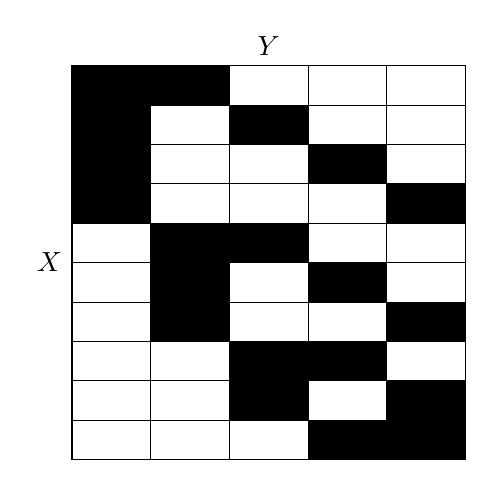
\begin{tikzpicture}[x=.5cm,y=1.cm,cm={0,-1,-1,0,(0,0)}]
\draw (0,0) -- (10,0) -- (10,5) -- (0,5) -- cycle;
\node[left] at (5,5) {$\mcal{X}$};
\node[above] at (0,2.5) {$\mcal{Y}$};
\draw[step=1,very thin] (0,0) grid (10,5);
\fill (0,4) -- +(1,0) -- +(1,1) -- +(0,1) -- cycle;
\fill (0,3) -- +(1,0) -- +(1,1) -- +(0,1) -- cycle;
\fill (1,4) -- +(1,0) -- +(1,1) -- +(0,1) -- cycle;
\fill (1,2) -- +(1,0) -- +(1,1) -- +(0,1) -- cycle;
\fill (2,4) -- +(1,0) -- +(1,1) -- +(0,1) -- cycle;
\fill (2,1) -- +(1,0) -- +(1,1) -- +(0,1) -- cycle;
\fill (3,4) -- +(1,0) -- +(1,1) -- +(0,1) -- cycle;
\fill (3,0) -- +(1,0) -- +(1,1) -- +(0,1) -- cycle;
\fill (4,3) -- +(1,0) -- +(1,1) -- +(0,1) -- cycle;
\fill (4,2) -- +(1,0) -- +(1,1) -- +(0,1) -- cycle;
\fill (5,3) -- +(1,0) -- +(1,1) -- +(0,1) -- cycle;
\fill (5,1) -- +(1,0) -- +(1,1) -- +(0,1) -- cycle;
\fill (6,3) -- +(1,0) -- +(1,1) -- +(0,1) -- cycle;
\fill (6,0) -- +(1,0) -- +(1,1) -- +(0,1) -- cycle;
\fill (7,2) -- +(1,0) -- +(1,1) -- +(0,1) -- cycle;
\fill (7,1) -- +(1,0) -- +(1,1) -- +(0,1) -- cycle;
\fill (8,2) -- +(1,0) -- +(1,1) -- +(0,1) -- cycle;
\fill (8,0) -- +(1,0) -- +(1,1) -- +(0,1) -- cycle;
\fill (9,1) -- +(1,0) -- +(1,1) -- +(0,1) -- cycle;
\fill (9,0) -- +(1,0) -- +(1,1) -- +(0,1) -- cycle;
\end{tikzpicture}
%
\caption{Schematic representation of Example~\ref{xpl5689}
for $n=5$ and $p=2$.}\label{fig5708}
\end{figure}

When considered as operators on~$L^2$ spaces, it is obvious that
$\pi_{XY}$ and~$\pi_{YX}$ are characterized by
$\big(\pi_{XY}f\big)(x) = p^{-1}\sum_{y\in x} f(y)$,
resp.\ $\big(\pi_{YX}g\big)(y) = \binom{n-1}{p-1}^{-1} \sum_{y\in x} g(x)$,
so that
\[ \big(\pi_{YXY}f\big)(y)
= \frac{1}{p} f(y) + \sum_{y'\neq y} \frac{p-1}{p(n-1)} f(y') .\]

Thus, on~$\ldb(Y)$, $\pi_{YXY}$ is nothing but the scalar operator $\frac{n-p}{p(n-1)}\mbf{I}$,
and therefore
\[\label{for7767} {\{X:Y\}} = \sqrt{\frac{n-p}{p(n-1)}} \]
by Proposition~\ref{pro7764} and Remark~\ref{rmk1265}.
\end{Xpl}


\paragraph{Weakly coupled particles}

\begin{Pro}\label{p8931}
Let~$V_1$ and~$V_2$ be potentials on~$\RR^n$, $n\geq 1$,
i.e.\ the~$V_i$ are real-valued measurable functions on~$\RR^n$
with $\int_{\RR^n} e^{-V_i(x)} \,\dx{x} < \infty$.
For $i\in\{1,2\}$, denote by~$\PP_i$ the probability measure on~$\RR^n$
proportional to~$e^{-V_i(x)}\dx{x}$, which is to be thought as
the law of the position $X_i$ of a particle $i$ subjected to the potential $V_i$.
Denote $\PP_\otimes \coloneqq \PP_1\otimes\PP_2$, which is the joint law of~$(X_1,X_2)$
in absence of interaction.

Now let~$W$ be an interaction potential on~$(\RR^n)^2$
such that $e^{\big{-[V_1(x_1)+V_2(x_2)+W(x_1,x_2)]}}$ is integrable;
denote by~$\PP$ the probability measure on~$(\RR^n)^2$ proportional to
$e^{-[V_1+V_2+W]} \,\dx{x_1}\dx{x_2}$,
which is the joint law of~$(X_1,X_2)$ in presence of interaction potential $W$.

Then, under the law $\PP$,
\[\label{f8367} \{X_1:X_2\} \leq \frac{\ecty_\otimes(e^{-W})}{\EE_\otimes[e^{-W}]} .\]
\end{Pro}

\begin{proof}
The law $\PP$ has density $h = e^{-W} \div \EE_\otimes[e^{-W}]$ w.r.t.~$\PP_\otimes$,
whence the result by Proposition~\ref{pro0651}.\linebreak[1]\strut
\end{proof}

\begin{Rmk}
Proposition~\ref{p8931} gives a rigorous sense to the intuition that two weakly coupled particles
must have nearly independent positions.
This is valid in a quite general setting,
in particular, $W$ does not have to be bounded.
\end{Rmk}


\paragraph{Non-reversible Markov chain}

\begin{Xpl}
Here is a example showing that the inequality in Proposition~\ref{cor0706}
is strict in general.
Consider the stationary Markov chain on~$\{1,2,3\}$ defined by
\[ P = \big(\!\big( \Pr[X_{k+1}=a | X_k=b] \big)\!\big)_{ab} =
\begin{pmatrix} 0&1/2&1 \\ 1&0&0 \\ 0&1/2&0 \end{pmatrix} ,\]
which has equilibrium measure~$(2/5,2/5,1/5)$.
Diagonalizing $P$ shows that
\[ P^t = \begin{pmatrix} 2/5&2/5&2/5 \\ 2/5&2/5&2/5 \\ 1/5&1/5&1/5 \end{pmatrix}
+ O(2^{-t/2}) ,\]
whence $\{ X_k:X_{k+t} \} = O(2^{-t/2})$ when~$t\longto+\infty$
by Proposition~\ref{pro3798}.
Yet ${\{X_k:X_{k+1}\}} = 1$, since the non-trivial events~${\{X_k = 1\}}$
and~${\{X_{k+1}=2\}}$ are equivalent (cf.\ Proposition~\ref{pro0699}).
\end{Xpl}


\paragraph{Hyperplanes in Ising's model}\label{parHyperplanesInIsingsModel}

As I told in Chapter~\ref{parMotivation},
the initial motivation of this work
was to understand the presence of $\rho$-mixing
in Ising's model (cf.\ \S~\ref{parIsingsModel});
in particular, I intended to re-get a result similar to Theorem~\ref{c6177}
by a more `natural' method.
That shall be achieved indeed in \S~\ref{parBackToIsingsModel}:
%
\begin{Thm}[Theorem~\ref{t3730}-(\ref{i3743a})]
For Ising's model on~$\ZZ^n$ in the completely analytical regime,
for all disjoint $I,J\subset\ZZ^n$,
\[\label{f46149} \{ \vec\omega_I : \vec\omega_J \} \leq
\exp\big[-\big(\psi'+o(1)\big) \, \dist(I,J)\big] ,\]
where $\psi'$ is the same as in Theorem~\ref{t4505}
and where the ``$o(1)$'' (to be understood ``as $\dist(I,J) \allowbreak {\longto \infty}$'') is uniform in~$I,J$.
\end{Thm}
%
If we apply that result to the case of parallel `hyperplanes' of~$\ZZ^n$
(I mean, sets of the form $\{t\}\times\ZZ^{n-1}$),
Formula~(\ref{f46149}) looks far less neat than Formula~(\ref{f2881}) in Theorem~\ref{c6177}.

That bound can however be improved by using Proposition~\ref{pro0281}.
Indeed, as we noticed in \S~\ref{parc6177}, the states of two parallel hyperplanes
are elements of some reversible stationary Markov chain.
Therefore, applying Corollary~\ref{cor5902} (in which we let~$k\to\infty$),
we get a result exactly similar to~(\ref{f2881}),
except that we have to replace $\psi$ by~$\psi'$ —recall that it is not known whether $\psi'=\psi$.



\section{Comparing \texorpdfstring{$\rho$}{rho}-mixing to other measures of dependence}

The material of this section is classical; most of it can be found for instance in
\cite[\S\S~3~\&~5]{Bradley-book}.
Here we will say that a sequence of pairs of $\sigma$-algebras $(\mcal{F}^n,\mcal{G}^n)$
is \emph{$\rho$-mixing} to mean that ${\{ \mcal{F}^n : \mcal{G}^n \}} \ab {\stackrel{n\longto\infty}{\longto} 0}$.

\subsection{\texorpdfstring{$\alpha$}{alpha}-mixing}\label{parAlphaMixing}

\begin{Def}
The \emph{$\alpha$-mixing} coefficient of two $\sigma$-algebras~$\mcal{F}$ and~$\mcal{G}$ is
\[ \alpha(\mcal{F},\mcal{G}) \coloneqq
\sup_{\substack{A\in\mcal{A}\\B\in\mcal{B}}} \big| \Pr[A\cap B] - \Pr[A]\Pr[B] \big| .\]
\end{Def}

Proposition~\ref{pro0699} shows that `$\rho$-mixing implies $\alpha$-mixing',
in the sense that one has $\alpha(\mcal{F},\mcal{G}) \leq A\big(\{\mcal{F}:\mcal{G}\}\big)$
for some universal function~$A \colon [0,1] \to [0,1]$
with $A(\rho) \stackrel{\rho\longto0}{\longto} 0$.

\begin{Rmk}
Saying that the correlation of two variables tends to~$0$ means that
their joint law tends in some sense to the product law.
When the variables are ranged in Polish spaces,
a common notion of convergence is weak convergence,
that is, convergence against all bounded continuous function.
%
\cite[Theorem~2.2]{Billingsley} states that weak convergence is implied
by~$\alpha$-mixing, hence by $\rho$-mixing.
The precise statement is the following:
if $(X^n,Y^n)_{n\in\NN}$ is a sequence of pairs of random variables
such that all the~$X_n$ (resp.~$Y_n$)
have the same law~$\Law(X)$ (resp.~$\Law(Y)$) in some Polish space $E$ (resp.~$F$), then
$\big(\alpha(X^n,Y^n) \stackrel{n\longto\infty}{\longto} 0\big) \ \Rightarrow
\ \big(\Law(X^n,Y^n)\stackrel{n\longto\infty}{\rightharpoonup}\Law(X)\otimes\Law(Y)\big)$.
\end{Rmk}

On the other hand, the following example shows that $\alpha$-mixing does not imply $\rho$-mixing:

\begin{Xpl}\label{x3993}
For~$\epsilon\in (0,1/2]$, define $(X^{\epsilon},Y^{\epsilon})$ in the following way:
\begin{itemize}
\item With probability $\epsilon$, one samples~$X^{\epsilon}$ and~$Y^{\epsilon}$ independently
with common law uniform on~$[0,\epsilon]$;
\item With probability $(1-\epsilon)$, one samples~$X^{\epsilon}$ and~$Y^{\epsilon}$ independently
with common law uniform on~$[\epsilon,1]$.
\end{itemize}
Then for all~$\epsilon>0$ one has $\{X^{\epsilon}:Y^{\epsilon}\}=1$,
since the non-trivial events~${\{X^\epsilon\leq\epsilon\}}$ and~${\{Y^\epsilon\leq\epsilon\}}$
are equivalent (cf.\ Proposition~\ref{pro0699}).
However it is easy to show that $\alpha(X^\epsilon,Y^\epsilon) = \epsilon-\epsilon^2
\stackrel{\epsilon\longto0}{\longto} 0$.
\end{Xpl}


\subsection{\texorpdfstring{$\beta$}{beta}-mixing}

Recall the definition of the $\beta$-mixing coefficient from the previous chapter
[Definition~\ref{def3167}].

\begin{Xpl}\label{xpl9506}
For~$\epsilon \in (0,1)$, consider two random sequences~$(X_i)_{i\in\NN}$ and~$(Y_i)_{i\in\NN}$
defined in the following way: $(X_i)_{i\in\NN}$ is a sequence of i.i.d.\ variables with uniform law on~$\{\pm1\}$,
and for each~$i\in\NN$, independently, one sets
$Y_i = X_i$ with probability $\epsilon$, and with probability $(1-\epsilon)$
one chooses~$Y_i$ uniformly on~$\{\pm1\}$.
Then all the~$(X_i,Y_i)$ are i.i.d.\ 
with $\Pr[X_i=\eta \enskip\text{and}\enskip Y_i=\theta] = (1+\eta\theta\epsilon)/4$
for all~$\eta,\theta\in\{\pm1\}$, thus $\{X_i:Y_i\} = \epsilon$
by Remark~\ref{rmk9549}, whence $\{\vec{X}:\vec{Y}\} = \epsilon$ by Theorem~\ref{pro1252}.
Yet $\Law(\vec{X},\vec{Y})$ and~$\Law(\vec{X})\otimes\Law(\vec{Y})$
are mutually singular for all~$\epsilon>0$.

This shows that $\rho$-mixing does not imply $\beta$-mixing,
and \emph{a fortiori} that there can be no kind of converse to Proposition~\ref{pro0651}.
\end{Xpl}


\subsection{Mutual information}

Recall the definition~(\ref{eq9402}) of mutual information.
\cite[Theorem~5.3(III)]{Bradley-book} states that mutual information controls
the $\beta$-mixing coefficient, so Example~\ref{xpl9506}, which
shows that $\rho$-mixing does not imply $\beta$-mixing in general,
shows that it does not imply mutual information to tend to~$0$ either.

Proposition~\ref{pro0651} suggests that, on the other hand,
maximal correlation could be controlled by mutual information,
but that is not true either: in Example~\ref{x3993} indeed,
$\{X^\epsilon:Y^\epsilon\} = 1$ for all~$\epsilon > 0$, but
\[ I(X^\epsilon;Y^\epsilon) =
\epsilon \ln (\epsilon^{-1}) + (1-\epsilon) \ln \big((1-\epsilon)^{-1}\big)
\stackrel{\epsilon\longto0}{\longto} 0 .\]

Mutual information measures the quantity of information shared by two random variables,
which explains intuitively the following property (\cite[Theorem~2.5.2]{CoverThomas}):
if $X\to Y\to Z$ is a Markov chain, then $I(Y;X,Z) \leq I(X;Y) + I(Y;Z)$.
Does a similar inequality hold for Hilbertian correlation?
In the Gaussian case, the answer is ``yes'' thanks to Theorem~\ref{pro1857}:
one gets that
\[ \{Y:X,Z\}^2 \leq
\frac{(1-\{Y:Z\}^2)\,\{X:Y\}^2 + (1-\{X:Y\}^2)\,\{Y:Z\}^2} {1-\{X:Y\}^2\{Y:Z\}^2}
\leq \{X:Y\}^2 + \{Y:Z\}^2 .\]
%
But that property does not hold in general, as the following example shows:

\begin{Xpl}\label{xpl1151}
Consider a Markov chain $X\to Y\to Z$,
where~$(Y,X)$ and~$(Y,Z)$ have the same law, which is the joint law described in Example~\ref{xpl5689}%
—the role of ``$Y$'' in that example being played here by~$Y$ in both cases.
Fix $y \in \mcal{Y}$; define event $A$ as ``$Y=y$''
and event $B$ as ``$y\in X\cap Z$''.
Then one computes that $\Pr[A] = n^{-1}$, while
\[ \Pr[B] = \frac{1}{n} + \frac{(p-1)^2}{n(n-1)} .\]
Since $A \subset B$, Proposition~\ref{pro0699}
then yields that
\[\label{for7766} \{Y:X,Z\} \geq \sqrt{\Pr[\C{B}]\Pr[A] \mathbin{\big/} \Pr[\C{A}]\Pr[B]}
= \left(\frac{(n-1)^2 - (p-1)^2} {(n-1)^2 + (n-1)(p-1)^2}\right)^{1/2} .\]

Comparing~(\ref{for7767}) and~(\ref{for7766}),
one sees that taking $n \gg 1$ and $1 \ll p \ll n^{1/2}$
makes~${\{X:Y\}}$ and~${\{Y:Z\}}$ arbitrarily close to~$0$
while $\{Y:X,Z\}$ gets arbitrarily close to~$1$.
\end{Xpl}

\begin{Rmk}
There are similar examples with $(X,Y,Z) = (Y_{-1},Y_0,Y_1)$ for a reversible Markov process $(Y_t)_{t\in\RR}$~\cite{perso}.
\end{Rmk}

